\chapter{モデルを使った研究の進め方}

\section{指針}
図\ref{fig:conceptual_diagram_statistics_research}には、統計モデルを使った研究の概念図を示した。
なんらかの生物学的問いに対して、それを観察するための実験デザインを構築し、現象からデータを取得する。
その現象がすでに観察されており、統計モデルが構築されていれば、そのモデルで標本を予測できるかを検証する。
もしも統計モデルや既存の研究がないならば、標本に適合するモデルを探索する\footnote{研究者らが普段使っている仮説検定は、ある一つのモデルが適合しないことを示しただけである。}。
そこで、どのようなモデルが適合するのかを探索する。
このとき、どのような分布関数が適合するのかや適当な母数やパラメータを推定する。
このモデルはデータに最もよく適合したモデルであるだろうから、適合モデルと呼ぶ。
構築した適合モデル$1$と生物学的な問いを元に新たな実験計画を設計し、その通りに実験を行う。
もしも標本2が適合モデルで対象にしていた特徴量を計測しているならば、適合モデル1の予測性能を測る。
予測できるならば、モデルの予測可能性が示される。
標本2に対する適応モデルを構築する。予測モデルと適応モデル2の差異を調べる。
予測モデルにより標本2を予測できないならば、その理由は次のものが想定できる。
\begin{enumerate}
    \item データが少数だったため、良い適合モデルを選べなかった(分布形の推定までできなかった等)
    \item 同様の実験条件を整えることができなかった(影響を受ける要因があったことを発見できた)
    \item 再現できない実験だった(実験デザインの見直し・再現できない研究の積み重ねを阻止)
\end{enumerate}

以上のプロセスを繰り返すことで、生物学の予測可能な領域を増やしていく。
%このプロセスに予測可能な領域を増やしていくことが生物を研究する上で重要な役割をになっている。(????)

\begin{figure}
    \begin{center}
        
\includegraphics[width=15cm]{./image/01_/conceptual_diagram/conceptual_diagram.006.png}
        \caption{統計モデルを使った研究のフロー図。}
        \label{fig:conceptual_diagram_statistics_research}
    \end{center}
\end{figure}

\subsection{どれが科学的成果だろうか}
1つ目の試験での成果は次のことになる。
\begin{enumerate}
    \item 標本があるモデルに適合しなかった($p$値・モデルの予測とデータが一致しないことを示す証拠)
    \item 標本に適合する適合モデル(モデルの分布形・母数)
\end{enumerate}

2つ目の試験における成果は次のことである。
\begin{enumerate}
    \item 標本$2$を適合モデル$1$が予測可能か。適合モデル1が予測にも使える。研究結果の予測可能性を確認。
    \item 適合モデル$1$が標本$2$を予測できなかった理由の探索
    \item 標本$2$の適合したモデル。適合モデル$2$と、適合モデル$1$の差異。
\end{enumerate}



\subsection{2群の検定問題}
標本が二つの群、A群B群となっており、これらの違いを定量的に求めると言う問題がある。
例えば、ある生物のオス、メスにおいて、体長が異なることを知りたいと言う問題である。
これまでは仮説検定を使い、2群の$t$検定などを使い、$p<0.05$であれば、違うという判定を行っていた。
これは、正規2モデル$M(\mu,\mu,\sigma^2,\sigma^2)$における統計量の予測と乖離していることを示しているにすぎない。
モデルは既存の知識を元に設定しているので、これまでの研究結果と異なることが示たと言うことである。

次の問いは、母数が同じモデルでは統計量が適合していないならば、標本に適合したモデルはどのようなものなのだろうか?
そこで、適合する統計モデルとその母数を探索する。
ここでは、対数尤度やAICなどを使う。ただし、これら指標の中で最適なものが将来的な標本の予測を良いものにするわけではない。単に相対的に当てはまりなどが良いだけである。

次に、モデルの性質を調べる。
母数の異なる二つの正規モデル$M_a,M_b$が適合したならば、そのモデルの差異を調べる。
例えば、統計量の出目の意味での類似度を示す検出力や、中心からの距離を分散で規格化した効果量などを求める。
例えば、効果量$d$が$0.001$程度であれば、$M_a,M_b$の中心は極めて近く、モデル$M_a$でどちらの群のデータも当てはまりが良いと判定できるかもしれない。
%これらの量から、片方の統計モデルが適合していると言うよりも、二つの正規モデルがより適合することが示せる。

次の試験において、生物学者はその生物が標高によって体長が異なるのではないかと言う問いを立てる。
さらに、オス・メスでその違いが顕著であるのではないかなどと考え、調査方法を構築する。
新たに得た標本において、オスメスそれぞれが$M_a,M_b$により標本を予測できているのかを調べる。
こうすることでモデルの予測能力と、一つ前の試験における研究の予測可能性を確認できる。
予測できないならば、なぜ予測できなかったのかを問い直すことになる。
さらに適合モデルなどを調べることになる。


\section{アヤメ(iris)に関する推論}
公開されているアヤメのデータを使って、研究の進め方について検討する。
このアヤメのデータでは$3$種(setosa,versicolor,virginica)のがく片の幅、がく片の長さ、花弁の幅、花弁の長さのデータが記録されている。
データサイズは、150で、種によって$50$ずつ記録されている。Pythonのライブラリsklearnから簡単にデータを呼び出せる。
\begin{lstlisting}
from sklearn import datasets
iris = datasets.load_iris()
\end{lstlisting}

\subsection{アヤメのがく弁の幅を予測するモデル}
ここでは、アヤメという植物が見つかったときどのようにモデルを構築するかを考える。
アヤメについてその種が3種類の分類が行われる前で、1種類であると考える。アヤメという植物を発見し、無作為に$150$個体を採集、がく弁の幅を計測したとする。
%我々が得ているのは、アヤメという植物のがく片の幅のデータ$150$個である。

我々は、がく弁の幅を予測するモデルを構築したい。
この目的を達成できるかはわからないが、一手目に行うのは、データに適合するモデルを探索することである。
データをみると、ある点を対称に同じくらいの数のデータがあることがわかる。
このことから、正規モデルが候補にあげられる。
データから平均と分散を求めると、$\bar{X}=3.05,\sigma=0.434$であった。
このことから、最尤正規モデルを構築する$M_a=M(3.05,\sigma^2=0.434^2)$である。
最尤正規モデルがデータに適合しているかをみる。
このモデルの予想では、$\mu$より大きいまたは小さいデータの個数は半数程度である\footnote{中央値と平均値が十分近ければ割合を調べなくてもいいかも}。
また、$\mu-\sigma \sim \mu+\sigma$の中にあるデータは$68\%$程度である。
表\ref{table:all_spael_width_table}がデータが予測にあっているかを示している。
どちらの指標も予想に合っている。
また、$>\mu$と$\mu<$となるデータの個数の比率も$1$に近い$1.24$であった。
これはモデルがデータに適合していることを示している。
\begin{table}[h]
    \caption{aa}
    \label{table:all_spael_width_table}
    \centering
    \begin{tabular}{lccccccc}
        %\toprule
        \hline
        {} &  $<\mu$ &  $>\mu$ &  Data Size &  $<\mu$ Rate &  $>\mu$ Rate &  $<\mu/>\mu$ & $\mu-\sigma\sim\mu+\sigma$\\
        %\midrule
        \hline
        All    &    83 &    67 &        150 &       0.55 &       0.45 &       1.24 & 0.673\\
        %\bottomrule
        \hline
    \end{tabular}
\end{table}

\begin{figure}
    \begin{center}
        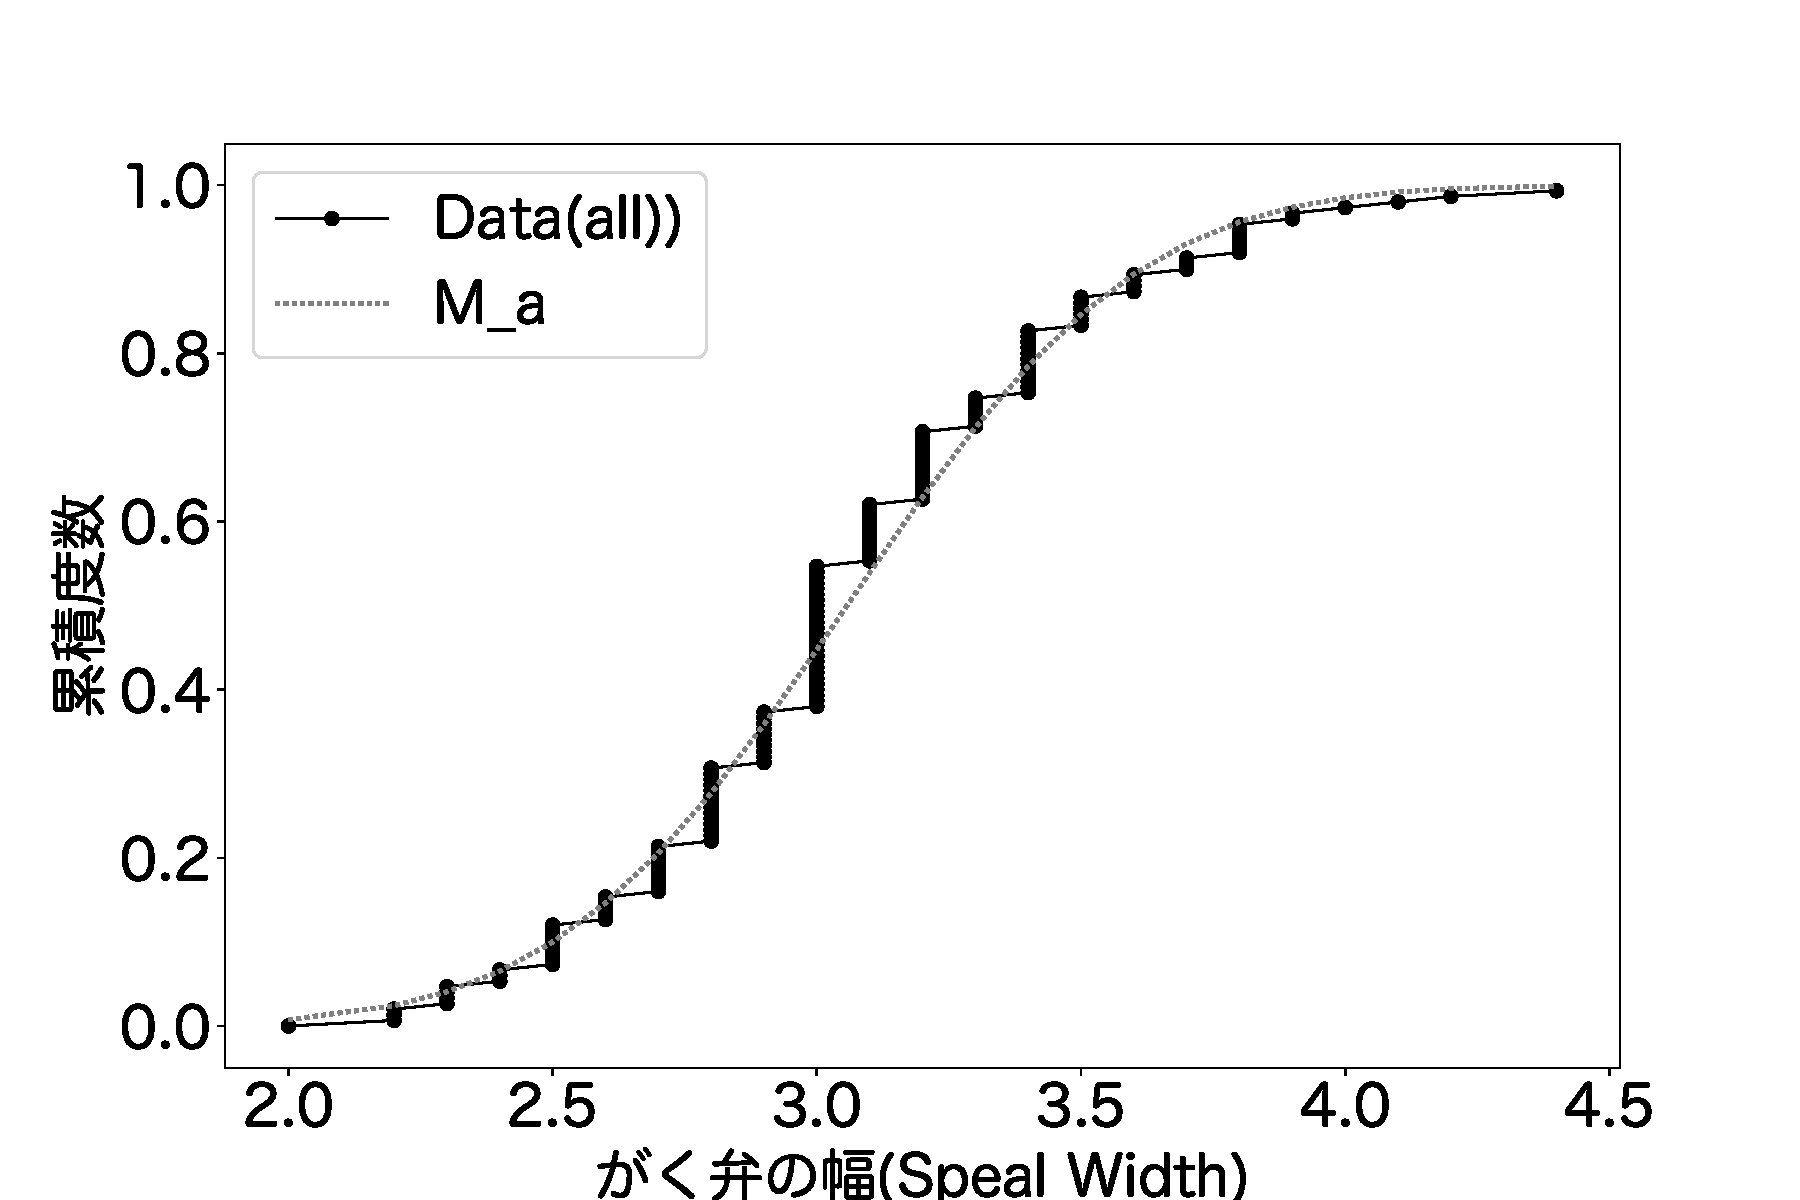
\includegraphics[width=15cm]{./image/15_/speal_width_all.pdf}
        \caption{データのがく弁の幅の累積度数(Data)と最尤モデルの累積度数$M_a$}
        \label{fig:all_speal_width_fig}
    \end{center}
\end{figure}

図\ref{fig:all_speal_width_fig}は、データの累積度数とモデルの累積度数を示している。
データとモデルの累積度数に関する予測がそれなりに一致していることがわかる。
このこともモデルがデータに適合していることを示唆している。

%アヤメについて統計モデルを使って予測する。
\subsection{アヤメの分類の細分化}
アヤメの分類を細分することになり、virginicaとそれ以外とすることになった。
これら二つのグループにおいて、がく弁の幅はこれまでに作ったモデル$M_a$により予測することができるだろうか。
新たにデータを取得し、モデルの予測とデータを比べることでモデル$M_a$の予測性能を測ることができる。
今回はデータを得るのが難しいので、もう一度同じデータを使い、モデルのデータに対する予測性能を測る\footnote{モデル構築に使ったデータを再び使うので、モデル$M_a$の予測の良さを測れていない}。
表\ref{table:speal_width_virig}がモデル$M_a$の予測に対する実際のデータの性質を示している。
virginicaとそれ以外はモデル$M_a$によって十分予測できていない。
モデル$M_a$の平均母数$\mu$より小さなものと大きなものの比が1より離れた値を取っている。
また、データの$68\%$が見つかるという予測をする区間には、$68\%$とはかけ離れた割合のデータが存在する。
図\ref{fig:virginica_speal_width_fig}には、モデル$M_a$とデータの累積度数を表示している。
モデル$M_a$の累積度数の上にデータの点がないことからも、モデルとデータが乖離していることが示唆される。
 

\begin{table}[h]
    \caption{アヤメ(virginicaとそれ以外)のがく弁の幅に関するデータの割合。モデル$M_a$の平均値を$\mu$としたとき、$\mu$より小さなデータの個数と割合($<\mu$、$<\mu$ Rate)。$\mu$より大きなデータの個数($>\mu$)と割合($>\mu$Rate)。$<\mu$と$>\mu$の割合。$\mu-\sigma\sim \mu+\sigma$の中にあるデータの個数($68\%$)と割合($68\%$Rate)。}
    \label{table:speal_width_virig}
    \centering
    \begin{tabular}{lrrrrrrrr}

        %\toprule
        \hline
        {} &  $<\mu$ &  $>\mu$ &  $<\mu$ Rate &  $>\mu$ Rate &  $<\mu/>\mu$ &  $68\%$ &  $68\%$Rate &  Data Size \\
        %\midrule
        \hline \hline
        virginica   &     8 &    42 &       0.16 &       0.84 &       0.19 &   27 &     0.54 &         50 \\
        others &    75 &    25 &       0.75 &       0.25 &       3.00 &   74 &     0.74 &        100 \\
        %All    &    83 &    67 &       0.55 &       0.45 &       1.24 &  101 &     0.67 &        150 \\
        %\bottomrule
        \hline
    \end{tabular}
\end{table}
    
\begin{figure}
    \begin{center}
        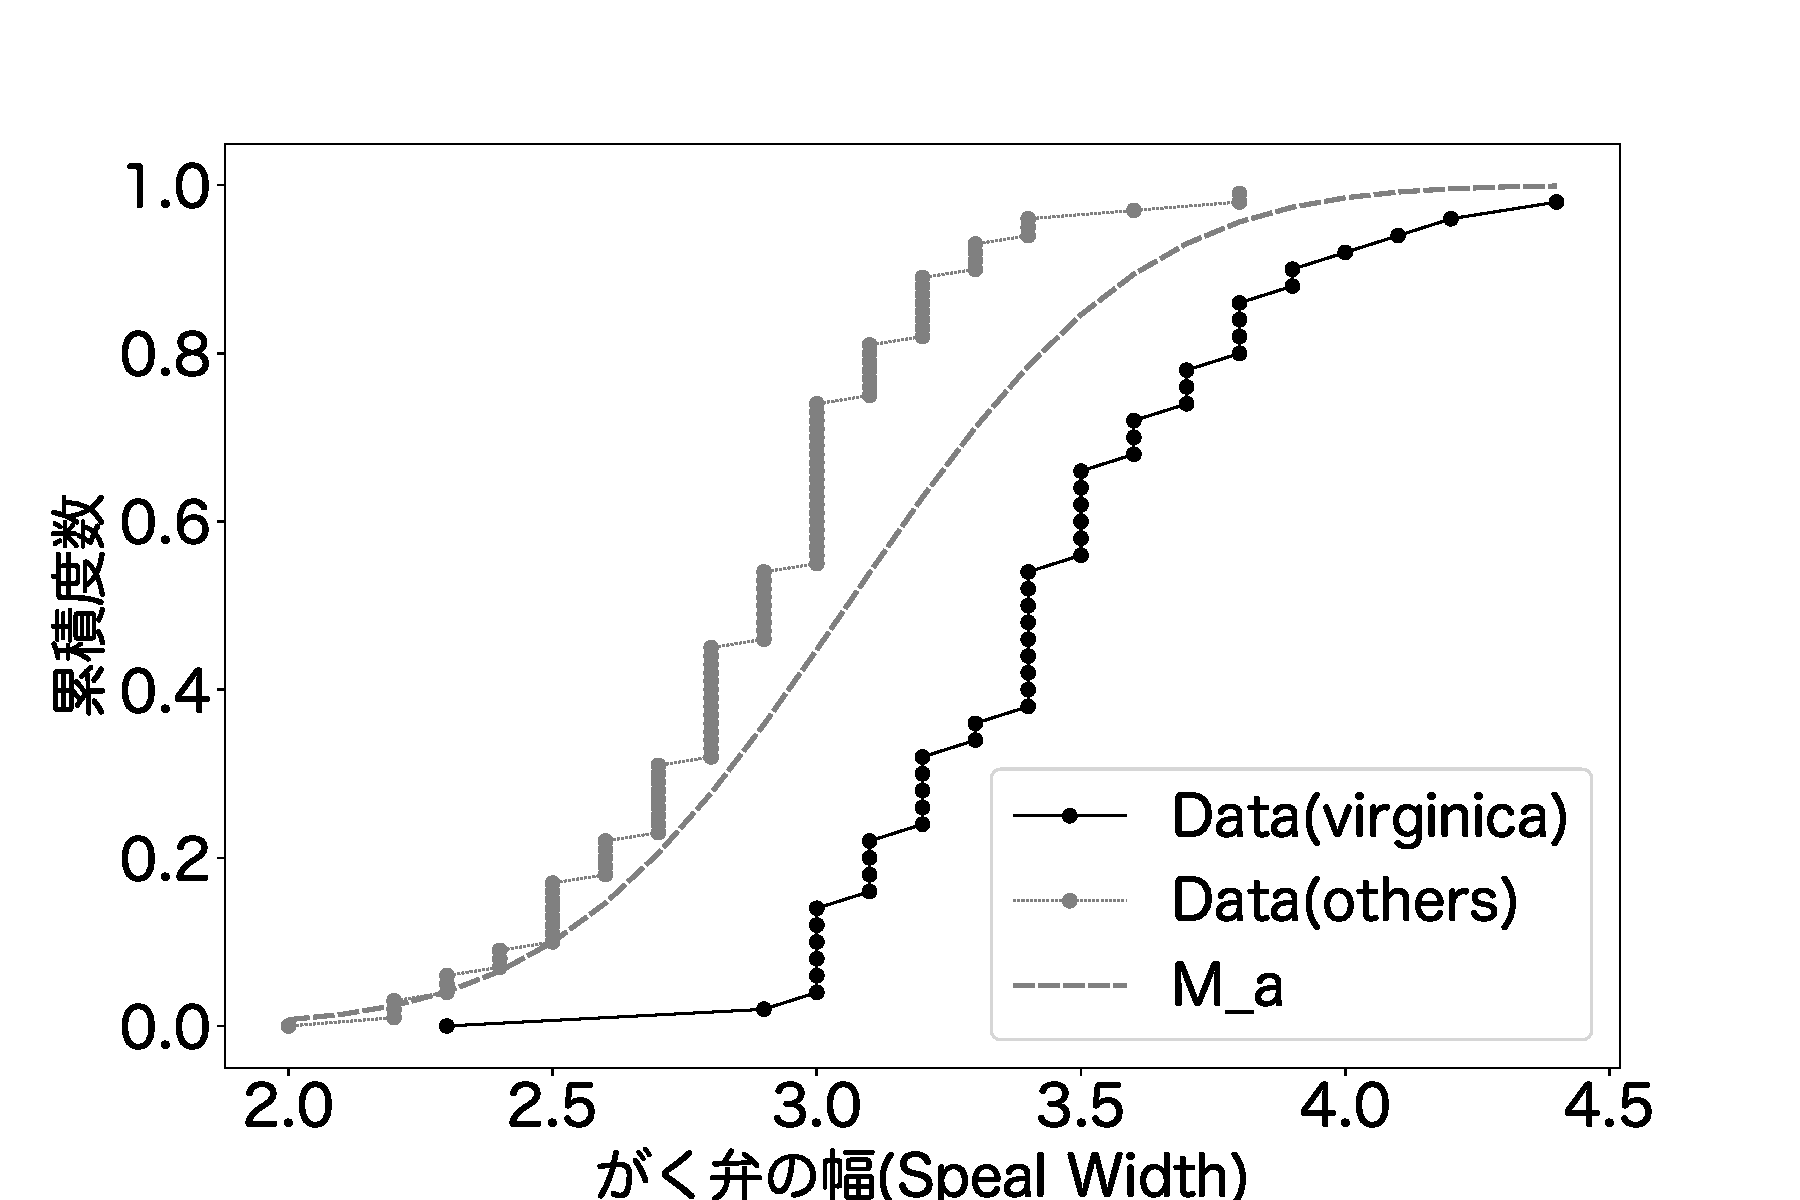
\includegraphics[width=15cm]{./image/15_/speal_width_viri.pdf}
        \caption{データのがく弁の幅の累積度数(Data)と最尤モデルの累積度数$M_a$}
        \label{fig:virginica_speal_width_fig}
    \end{center}
\end{figure}

モデル$M_a=M(\mu=3.05,\sigma^2=0.434^2)$における統計検定量も利用する。
次のことがわかっている。
\begin{equation*}
    Z = \frac{\sqrt{N}(\mu-\bar{x})}{\sigma} \sim N(0,1)
\end{equation*}
統計検定量$Z$を計算した結果が表\ref{table:speal_width_Z}である。
$Z$の絶対値は、$2$より大きくモデルとデータが乖離していることがわかる。

\begin{table}
    \caption{統計検定量$Z$}
    \label{table:speal_width_Z}
    \centering
    \begin{tabular}{lccc}
        \hline
        {} &   $\bar{x} $ &  $\sigma$  &     Z \\
        \hline \hline
        virginica &  3.43 &  0.38 & -6.03 \\
        others    &  2.87 &  0.33 &  4.27 \\
        $M_a$ & 3.05 & 0.434 & - \\
        \hline
    \end{tabular}
\end{table}

これらのことから、モデルの改訂をした方が良いことが示唆される。

以上のことは論文においては、統計統計量より偏った値が得られる確率($p$値)または$p<0.05$が報告される。
すでに議論した通り、$p$値だけでモデルとデータの乖離を検証すると、モデルの予測性能が過度に低いと判定されることがある。さまざまな指標を元にモデルの予測性能を測るべきである。

\subsection{新たなモデルの構築}
virginicaとothersに適合するモデルをそれぞれ構築する。
累積分布はどちらも正規分布的になっている。$M_a$を構築するときと同じようにそれぞれの平均と分散を求め(表\ref{table:speal_width_Z}の通りである)、データが平均に対して対称に分布していること、$\mu-\sigma\sim\mu+\sigma$の間にあるデータが$68\%$程度であるかを確かめる。

\begin{table}
    \caption{新たなモデル$M_v,M_o$による予測とデータの適合具合}
    \label{table:speal_width_replace_model}
    \begin{tabular}{lrrrrrrr}
        %\toprule
        \hline
        {} &  $<\mu$ &  $>\mu$ &  $<\mu$Rate &  $>\mu$Rate &  $<\mu/>\mu$  &  $68\%$Rate &  Sample Size \\
        %\midrule
        \hline \hline
        0 &   28 &   22 &     0.56 &     0.44 &      1.27 &     0.72 &           50 \\
        1 &   46 &   54 &     0.46 &     0.54 &      0.85 &     0.72 &          100 \\
        %\bottomrule
        \hline
    \end{tabular}
\end{table}   

表\ref{table:speal_width_replace_model}には、新たなモデル$M_v$および$M_o$の予測とデータの適合具合を示している。
どの指標もモデルの予想と一致しており、モデルがデータと適合していることを示唆している。

\begin{figure}
    \begin{center}
        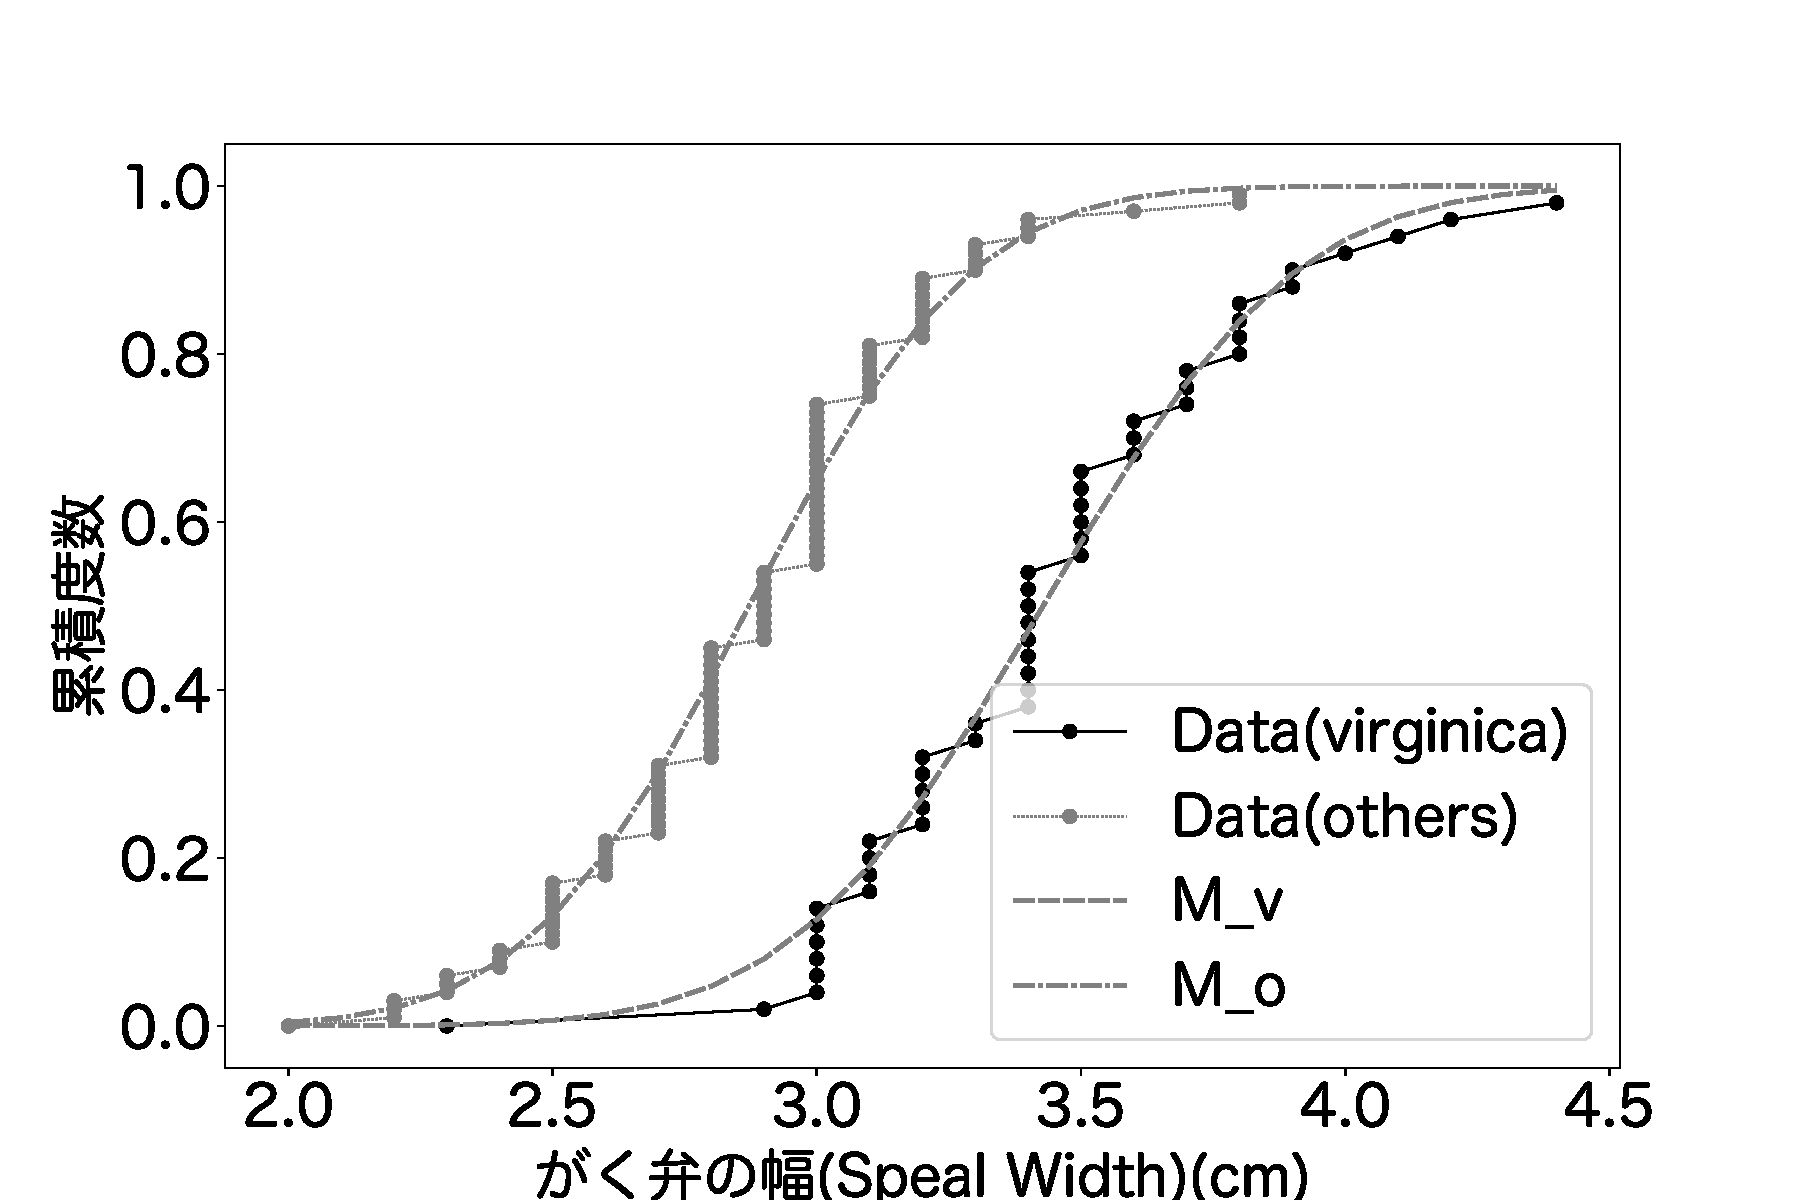
\includegraphics[width=15cm]{./image/15_/speal_width_viri_model.pdf}
        \caption{データのがく弁の幅の累積度数(Data)と最尤モデルの累積度数$M_v,M_o$}
        \label{fig:speal_width_viri_model}
    \end{center}
\end{figure}

図\ref{fig:speal_width_viri_model}はモデルの累積度数とデータの適合具合を示している。
それぞれのモデルがそれぞれデータをよく予測していることがわかる

\subsection{更なる生物学的な種の細分化}
アヤメのothersについても細分化することになったsetosa,versicolorである。これらについて予測モデル$M_v$は良い予測をするかを調べ、予測できないと判断したのなら、モデルを構築し直す。

これまでのアヤメに関する議論はなかったことにして、まっさらな状況でモデルを使う方法について考える。
状況設定として、これまで同一だと分類されていたアヤメを2種類に分けるということになった。
この2種類のがく弁の幅ついてこれまでと同じモデルを使って予測できるだろうか。
この$2$種類を予測するモデルとして、正規2モデル$M_2=M(\mu,\mu,\sigma^2,\sigma^2)$とし、$M_2$によりがく弁の幅が予測できるかを考える。
同じアヤメという分類に属するのだから、がく弁の幅も同じ程度だろうと考え、$\mu$が同一のモデルを選んだ\footnote{頻度論を元にした生物学の教科書では、母数を同一にするのは、そうでないことを示すため(背理法)と説明されることがある。本書の方針とは異なる。本書では、これまで同一だと思われていたアヤメの分類が増えたので、それまではがく弁についてもある統計モデル$M$で予測されていたと言う前提があったとする。実際にデータと適合モデルが既存研究において提案されてたとする。母数が同じと考えられていたモデルで予測可能であるかを調査するために、モデルの統計量に関する予測を利用する。この論証は背理法ではない。}。また、正規分布を仮定したのも、これまでアヤメのがく弁は正規モデルで予測していたからである\footnote{と言う設定の上で推論を進めていく。実際には、既存研究でどのように扱われていたかを調べる必要がある。もしも指数分布で推測していたなら、分布形や統計検定量を変える。既存の研究成果で予測ができるのかを調べるためである。既存の予測が当たらなかったら、新たなモデルを提案する。既存のモデルが予測には適さないことや新しいモデルの提案は科学的な成果である。報告するべき事柄である。}。

\begin{equation*}
    t = \frac{\bar{x}-\bar{y}}{s\sqrt{\frac{1}{m} + \frac{1}{n} }} \sim t_{m+n-2}
\end{equation*}
ここで、$s^2=\frac{(m-1)s_x^2+(n-1)s_y^2}{m+n-2}$である。
パラメータについては、表\ref{fig:seto_versi_speal_w_summary}にある通りである。
これを元に計算すると、$t=9.45$程度である。
このことから、モデル$M_2$では予測しにくいと考えられる。

\begin{table}
    \caption{setosa、versicolorのがく弁の幅のデータの統計量}
    \label{fig:seto_versi_speal_w_summary}
    \centering
    \begin{tabular}{lrrr}
        \hline
        {} &  Ave. &  Sigma &   N \\
        \hline \hline
        setosa     &  3.43 &   0.38 &  50 \\
        versicolor &  2.77 &   0.31 &  50 \\
        setosa and versicolor &  3.10 &   0.48 &  100 \\
        \hline
    \end{tabular}
\end{table}

最尤モデル$M=M(3.10,0.48^2)$のデータへの適合具合を見る。累積度数はモデルと離れていることがわかる(図\ref{fig:speal_width_setosa_versi_model})。
以上から、$M_2$ではデータと適合していないことがわかる。


\begin{figure}
    \begin{center}
        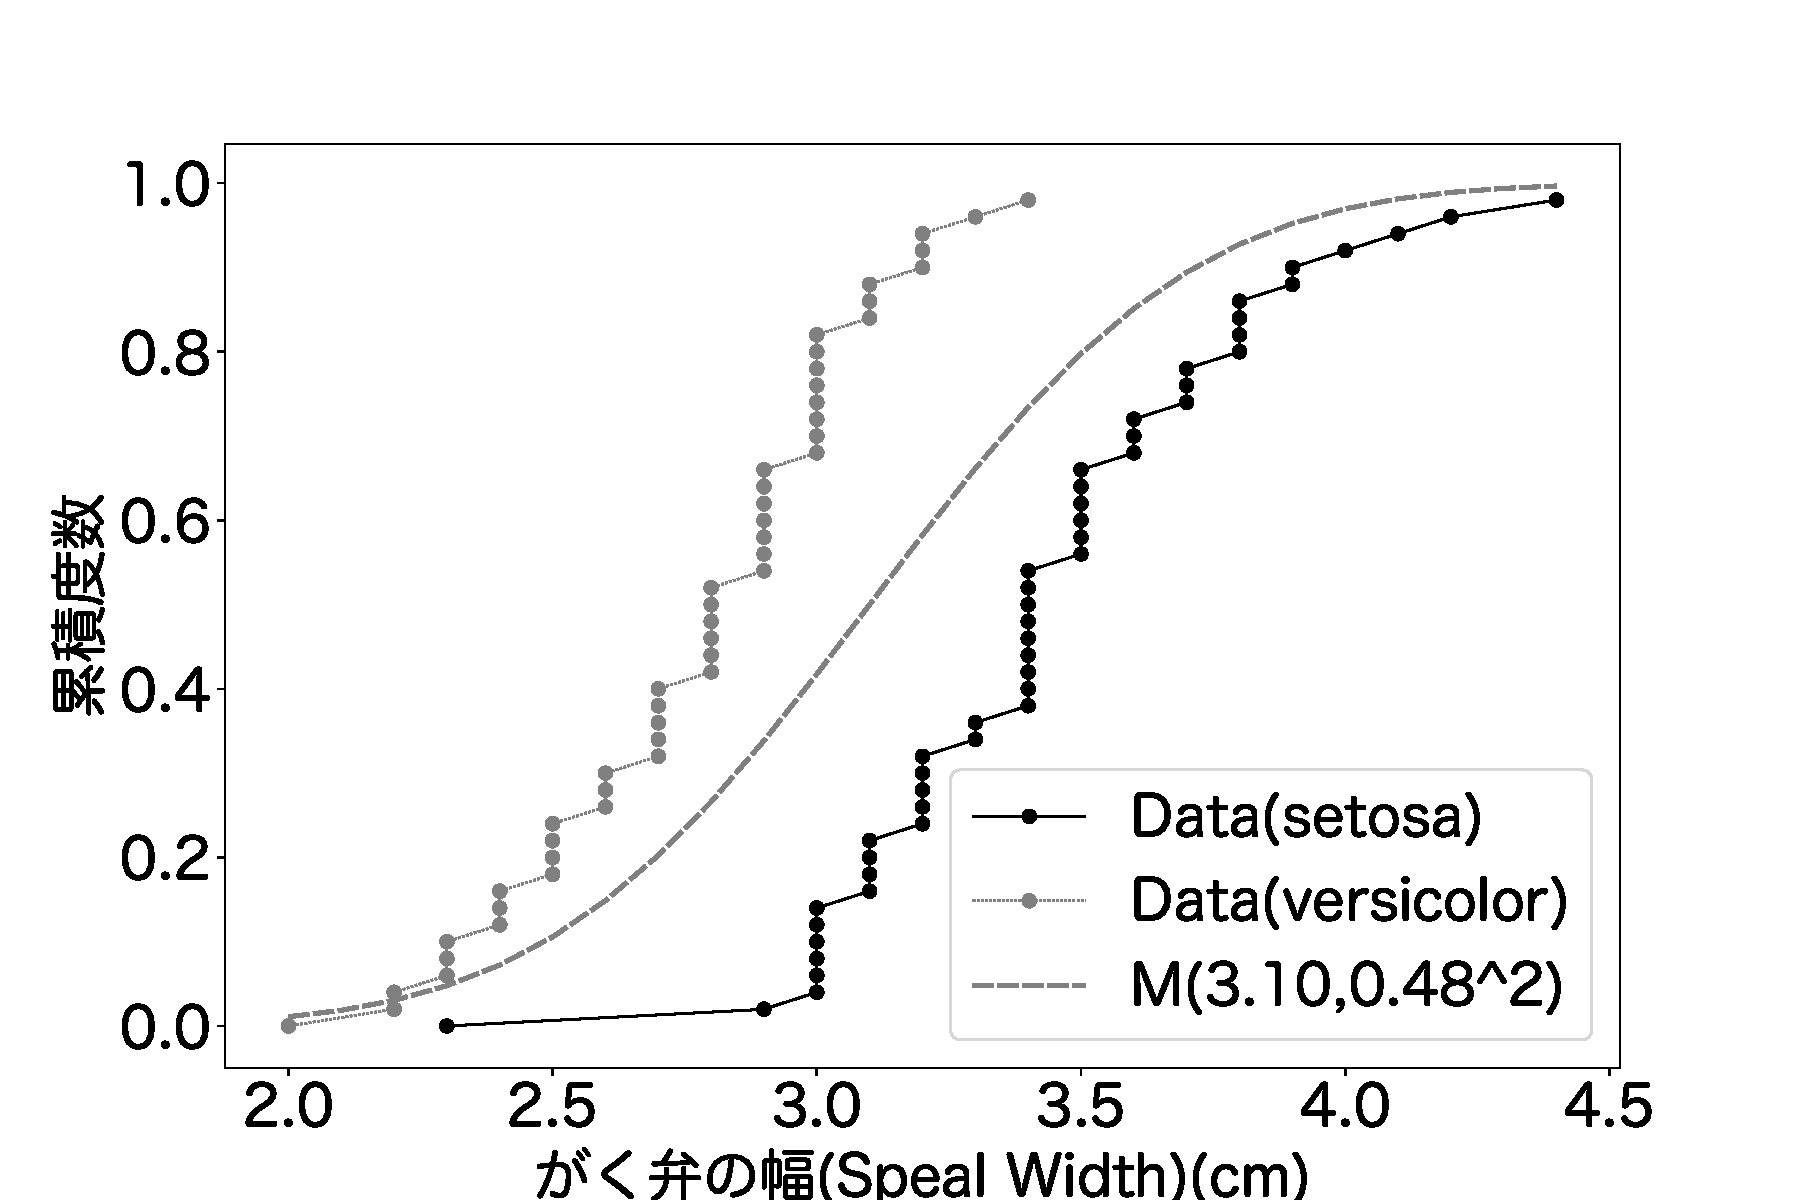
\includegraphics[width=15cm]{./image/15_/speal_width_seto_versi_model.pdf}
        \caption{データのがく弁の幅の累積度数(Data)と最尤モデルの累積度数$M$}
        \label{fig:speal_width_setosa_versi_model}
    \end{center}
\end{figure}


二つのモデルを構築し、それぞれがversicolorとsetosaのデータに適合するかを調べる。
面倒なので勝手にやってくれ。


\subsubsection{種が細分化されたならば、モデルも更新すべき?}
種は細分化されたが予測モデルは同一のものを使ってもいいという判断を下すこともある。
言い換えれば、生物学的な特徴を元に種を細分化したが、別の特徴は同じモデルで予測できるということもある。


\section{ダニの個体数}
grouseticksはライチョウのひなの頭についているダニの個体数をスコットランド(北緯$57$度$7$分、西経$3$度$19$分)で調べたデータである。
Pythonでも呼び出すことができる。

\begin{lstlisting}
    import statsmodels.api as sm
    data = sm.datasets.get_rdataset("grouseticks", "lme4").data
    ticks = data['TICKS'].values
\end{lstlisting}

\begin{SMbox}{カウントデータだからポアソン分布}
    \begin{quote}
        カウントデータならポアソン回帰で!\footnote{P.19 \url{https://kuboweb.github.io/-kubo/stat/2011/y/skubostat2011y.pdf}}\\
        • もしこの観測データ (縦軸) がカウントデータだったら?\\
        まずい点: 等分散ではないに直線回帰?\\
        まずい点: モデルによる予測は「負の個体密度」?\\
    \end{quote}
    カウントデータだからポアソン分布を仮定しよう。その理由は、正規分布などであれば、負の個体数が出てくるので、現象をよく予測できていないと言うことが挙げられている。ここでいうカウントデータはある一定時間に起きた事象の回数のことではなく、種子の個数のことである。

    このことは本書では推奨しない。
    予測が現象を反映していないことは、大きな問題ではない。例えば、身長の分布の推定に正規分布を使った。正規分布の推定では負の身長は、非常に低い確率で出現する。これは物理的にあり得ない。では、この仮定がダメなのかと言えばそんなことはない。あり得ない部分は無視して、予測したいことが予測できれば問題にならない。

    また、大学入試の共通テストの得点分布はおよそ正規分布で推測可能な形になっている。このことからテストの得点は正規分布すると考えてはいけない。
    実際にテストを作って、学生に解かせてみると、その分布は正規分布とは程遠い。授業の得点を予測するのに正規分布は仮定しないほうがいいことがわかる。状況に応じて予測できそうなモデルを構築する必要があることを示唆している。

    カウントデータなのだからポアソン分布を仮定することは本書では勧めない。データに適合しないならば、より多くの適合しそうなモデルを探索してみることを勧める\footnote{分散も平均も変化するデータなので、正規分布を仮定したモデルだと計算が破綻するのかもしれない。このことを私は調べてない。}。また、適合する分布が見つからないこともある。
\end{SMbox}




\if 0
TODO: モデルの分布に変更が必要な場合が考えられるデータが欲しい
TODO: データ数が大きくて、$p<0.0000$になるので乖離している状況。その上で、予測には問題がないことを示すデータ。身長のデータがこれに当たるかな。
\fi

